The simulations done by the authors regarding system \ref{eq:System2} and taking into account a possible birth rate perturbation, are shown in Figure \ref{birth1}.  
\begin{figure}[h!]
    \begin{subfigure}{0.5\textwidth}
        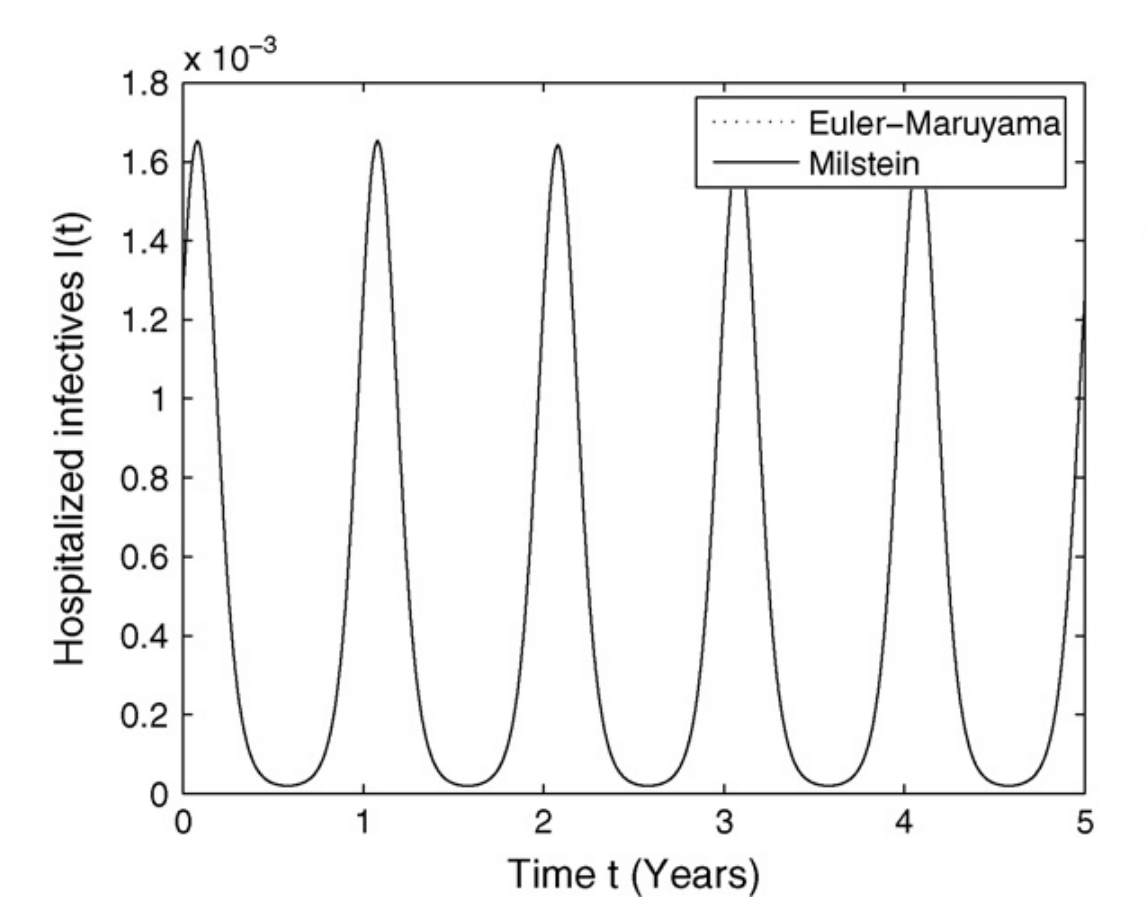
\includegraphics[width=\linewidth]{IMG/Euler_Maruyama_birth.png}
        \caption{}
    \end{subfigure}
    \begin{subfigure}{0.5\textwidth}
        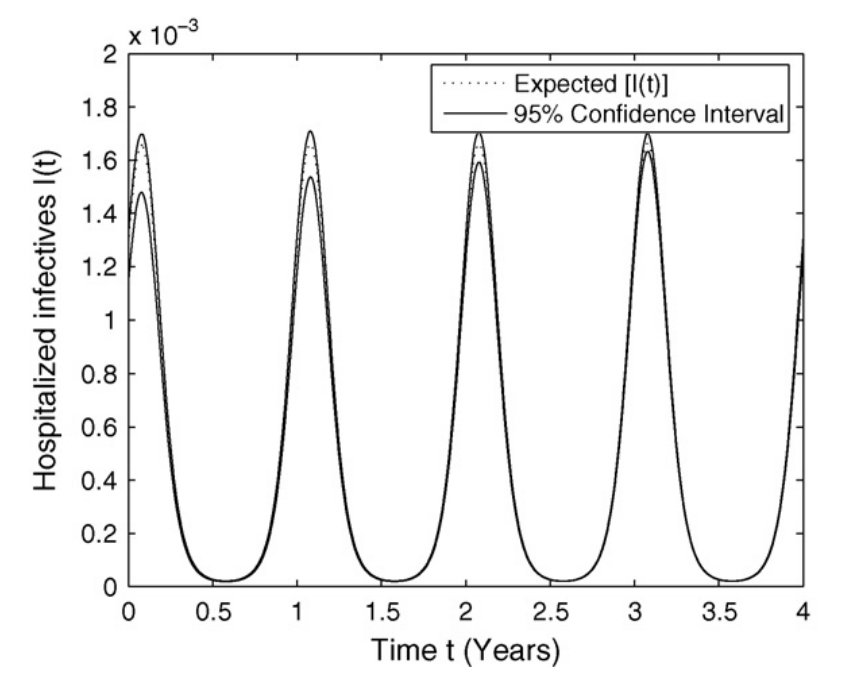
\includegraphics[width=\linewidth]{IMG/birth_rate_is_perturbated1.png}
        \caption{}
    \end{subfigure}
    \caption{(a)Comparison between the Milstein and Euler-Maruyama stochastic scheme in regard to the infected sub population I(t) over a single simulation with birth rate perturbation.(b) Confidence intervals and expected behavior for the infected sub population I(t) when the birth rate is perturbed at 100\% ($\alpha$ = 0.009).}
    \label{birth1}
\end{figure}

In the same figure we can see the 95\% confidence interval and anticipated trajectory for the infected sub population I(t) are depicted through Monte-Carlo simulations. Despite the substantial magnitude of these environmental stochastic perturbations, the infected population exhibits a nearly identical periodic behavior compared to the deterministic model presented before.

\begin{figure}[ht]
  \centering
  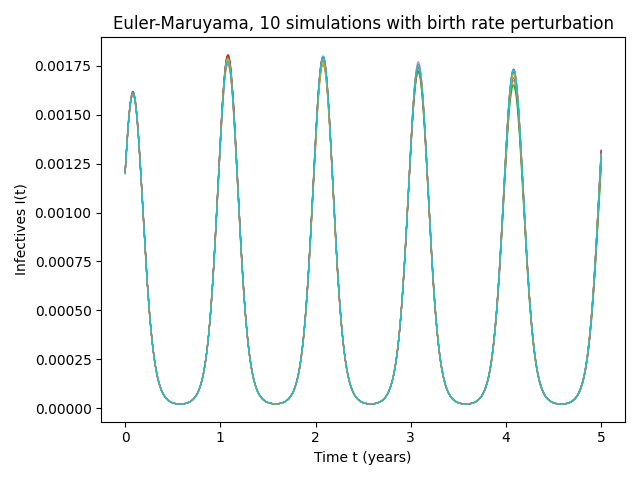
\includegraphics[width=0.8\textwidth]{IMG/birth_aphabig_I(t).png}
  \caption{Euler-Maruyama stochastic graph in regard to the infected sub population I(t) with birth rate perturbation over multiple simulations.}
  \label{birth2}
\end{figure}

Similar results were obtained by our implementation as shown in Figure \ref{birth2}, where it is evident that even after multiple simulations there is not much change from the deterministic model.
